\documentclass[12pt]{article} 
\usepackage{graphicx} 
\usepackage{titlesec}

% Replace `letterpaper' with `a4paper' for UK/EU standard size
\usepackage[a4paper,top=2cm,bottom=2cm,left=3cm,right=3cm,marginparwidth=1.75cm]{geometry}

% Useful packages
\usepackage{amsmath}
\usepackage{graphicx}
\usepackage{tabularx} % Include the tabularx package
\usepackage{hyperref}
\usepackage{caption}
\usepackage{subcaption}
\usepackage{caption}
\usepackage{subcaption}
\usepackage{placeins}
\usepackage{amssymb} % This package defines \mathbb
\usepackage{booktabs} % For professional looking tables
\usepackage{amsfonts}

% Center section headings
\titleformat{\section}
  {\normalfont\Large\bfseries}
  {\thesection}
  {1em}
  {}
 

\begin{document}

\begin{titlepage}
\centering
\vspace{0.5cm}
{\Huge\bfseries Variational Autoencoders\par}

\vspace{0.5cm} % Adds vertical space
{\Large SAiDL 2024 Assignment}

\vspace{1.5cm}
{\Large Sasmit Datta}
\end{titlepage}

%%%%%%%%%%%%%%%%%%%%%%%%%%%%%%%%%%%%%%%%%%%%%%%
\section{Introduction}
Variational Autoencoders (VAEs) represents a seminal approach in the field of generative models, allowing the learning of complex data distributions like images through latent space exploration. This report entails an analysis of two distinct VAEs
with the same architecture but different prior distributions: $\mathcal{N}(0,1)$ and $\mathcal{N}(1,2)$.

Furthermore, I try to improve generations from $\mathcal{N}(1,2)$ by deployment of various loss functions - \textbf{BCE}, \textbf{MAE}, \textbf{MSE}, \textbf{perceptual loss}, and \textbf{weighted perceptual loss with additional loss term} and other methods like changing initialization.

I also implement a \textbf{FID Score Calculator} to compare the quality of generations from different models.

%%%%%%%%%%%%%%%%%%%%%%%%%%%%%%%%%%%%%%%%%%%%%%%
\section{VAEs}
VAEs consist of an encoder which learns to map data to a latent distribution and a decoder that reconstructs data from this distribution.

\subsection{Formulation}
Given data $\mathbf{x}$ with latent variables $\mathbf{z}$, the encoder approximates the true posterior $p(\mathbf{z}|\mathbf{x})$ with a variational approximation $q_{\phi}(\mathbf{z}|\mathbf{x})$. The decoder then reconstructs the data from the latent space, modeling $p_{\theta}(\mathbf{x}|\mathbf{z})$. The VAE is trained by maximizing the evidence lower bound (ELBO) on the marginal likelihood of each data point:
$$\mathcal{L}(\theta, \phi; \mathbf{x}) = -\mathbb{E}_{q_\phi(\mathbf{z}|\mathbf{x})}[\log p_\theta(\mathbf{x}|\mathbf{z})] + D_{\text{KL}}(q_\phi(\mathbf{z}|\mathbf{x}) \| p(\mathbf{z}))$$
Here, $D_{\text{KL}}$ denotes the Kullback-Leibler divergence, providing conditioning by penalizing the deviation of $q_\phi(\mathbf{z}|\mathbf{x})$ from the prior $p(\mathbf{z})$. So when we pass samples from our prior $p(\mathbf{z})$ to the decoder, we can generate novel data.
\subsection{Reparameterization Trick}
The reparameterization trick enables gradient-based optimization of VAEs by expressing the random variable $\mathbf{z}$ as a deterministic function of $\mathbf{x}$ and random variable $\epsilon$. 
%%%%%%%%%%%%%%%%%%%%%%%%%%%%%%%%%%%%%%%%%%%%%%%
\section{Model}

\subsection{Architecture}
Fig \ref{fig:architecture} is the architecture of the model used.
\begin{figure}[h]
\centering
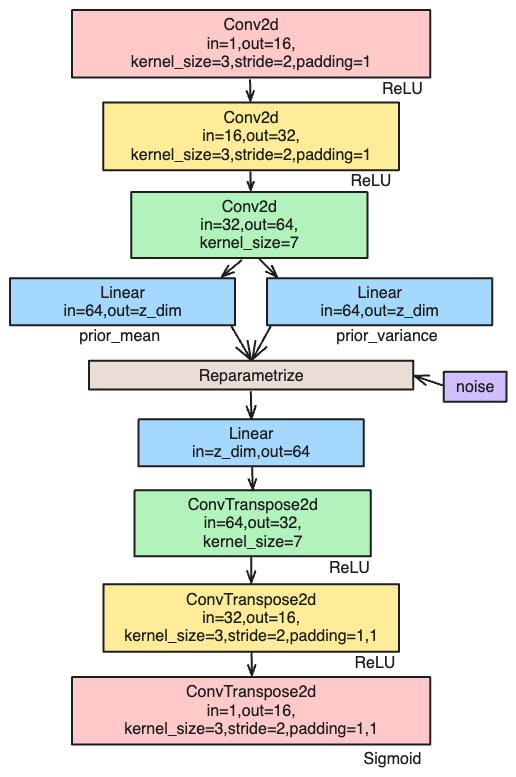
\includegraphics[width=0.5\linewidth]{report_images/architecture.png}
\caption{\label{fig:architecture}VAE Architecture}
\end{figure}

\subsection{Common Hyper-parameters}
Common hyper-parameters I use to train these models are:
\begin{itemize}
\item Optimizer: \textbf{Adam} with default Pytorch settings except for the learning rate.
\item Learning Rate = 0.0001
\item Epochs = 15
\item Batch Size = 64
\item Latent Dimension = 2
\end{itemize}

%%%%%%%%%%%%%%%%%%%%%%%%%%%%%%%%%%%%%%%%%%%%%%%
\section{Perceptual Loss}
Perceptual loss evaluates the similarity between images using high-level feature representations from a pre-trained CNN, focusing on perceptual rather than pixel-wise differences.

Perceptual loss is defined as the difference in feature representations from a CNN between a generated image $\mathbf{\hat{x}}$ and a real image $\mathbf{x}$:

\begin{equation}
\mathcal{L}_{\text{perceptual}}(\mathbf{x}, \mathbf{\hat{x}}) = \sum_{l} \| \Phi_l(\mathbf{x}) - \Phi_l(\mathbf{\hat{x}}) \|_2^2
\end{equation}
where $\Phi_l$ represents the activation of the $l$-th layer of the CNN.

\subsection{Weighted Perceptual Loss with Additional Loss Term}
Given reconstructed image $\mathbf{\hat{x}}$ and a target image $\mathbf{x}$, the weighted perceptual loss incorporating an additional loss term can be formulated as:

\begin{equation}
\mathcal{L}(\mathbf{x}, \mathbf{\hat{x}}) = \lambda \sum_{l} \| \Phi_l(\mathbf{x}) - \Phi_l(\mathbf{\hat{x}}) \|_2^2 + \mathcal{L}_{\text{additional}}(\mathbf{x}, \mathbf{\hat{x}})
\end{equation}
where $\lambda$ is the weighting factor, $\Phi_l$ denotes the activation of the $l$-th layer in a pre-trained CNN, and $\mathcal{L}_{\text{additional}}$ represents the additional loss term, such as binary cross-entropy (BCE) or mean squared error (MSE).

\subsection{Implementation}
For the pre-trained CNN, I use a straightforward MNIST classifier (Fig \ref{fig:classifier}) trained over the course of \textbf{5 epochs} using an \textbf{Adam optimizer} with \textbf{learning rate} set to \textbf{0.001} and a \textbf{batch size} of \textbf{64}, getting a \textbf{99\% accuracy} on the test set. I use the features of \textbf{2'nd} and \textbf{4'th ReLU activations} of this model to calculate the perceptual loss. $\boldsymbol{\lambda}$ is set to \textbf{0.01} for the \textbf{weighted perceptual loss with an additional loss term} in my experiments.

\begin{figure}[h]
\centering
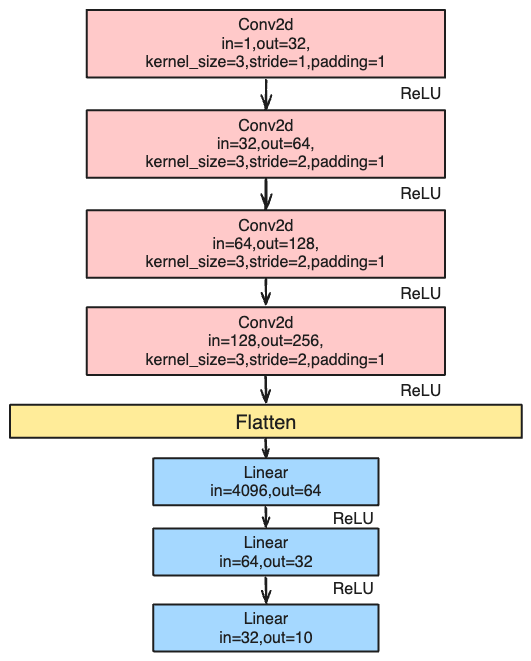
\includegraphics[width=0.5\linewidth]{report_images/classifier.png}
\caption{\label{fig:classifier}Perceptual Loss MNIST Classifier}
\end{figure}

%%%%%%%%%%%%%%%%%%%%%%%%%%%%%%%%%%%%%%%%%%%%%%%
\section{Baselines}
I used the \texttt{rsample()} method of \texttt{torch.distributions.normal.Normal()} to sample latent vectors, the native KL-Divergence method to calculate $D_{\text{KL}}(q_\phi(\mathbf{z}|\mathbf{x}) \| p(\mathbf{z}))$ and BCE Loss for $\mathcal{N}(0,1)$ and $\mathcal{N}(1,2)$ baseline models.
\begin{equation}
\text{BCE} = -\sum_{i=1}^{N} \left[ y_i \log(\hat{y}_i) + (1 - y_i) \log(1 - \hat{y}_i) \right],
\end{equation}
where \(N\) is the number of pixels in the image, \(y_i\) represents the true pixel values of the original image, and \(\hat{y}_i\) denotes the predicted pixel values from the reconstructed image. All the latent space plots can be found in Section \ref{latent_spaces}.

\subsection{$\boldsymbol{\mathcal{N}(0,1)}$ Prior}
For an isotropic gaussian prior, and a gaussian posterior whose parameters we have to predict, $D_{\text{KL}}(q_\phi(\mathbf{z}|\mathbf{x}) \| p(\mathbf{z}))$ can be written as:
\begin{equation}
D_{\text{KL}}(q_\phi(\mathbf{z}|\mathbf{x}) \| p(\mathbf{z})) = -\frac{1}{2} \sum_{j=1}^{n} \left[1 + \log\sigma_j^2 - \sigma_j^2 - \mu_j^2  \right]
\end{equation}
where $n$ is the dimension of the latent space.  The model's interpolation and latent space plots can be found in Fig \ref{fig:inter_normal} and Fig \ref{fig:latent_normal} respectively. 

\begin{figure}[h]
\centering
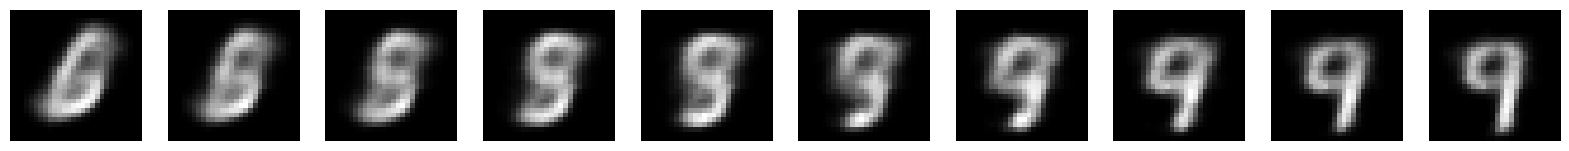
\includegraphics[width=1\linewidth]{report_images/normal_vae/interpolation.png}
\caption{\label{fig:inter_normal}Interpolation: $\mathcal{N}(0,1)$ Prior}
\end{figure}



\subsection{$\boldsymbol{\mathcal{N}(1,2)}$ Prior}
For a $\mathcal{N}(1,2)$ prior, and a gaussian posterior whose parameters we have to predict, $D_{\text{KL}}(q_\phi(\mathbf{z}|\mathbf{x}) \| p(\mathbf{z}))$ can be written as:
\begin{equation}
D_{\text{KL}}(q_\phi(\mathbf{z}|\mathbf{x}) \| p(\mathbf{z})) = -\frac{1}{2}\sum_{j=1}^n \left[ 1 - 2\log2 + \log\sigma_j^2  - \frac{1}{4}\sigma_j^2 - \frac{1}{4}(1 - \mu_j)^2 \right]
\end{equation}
where $n$ is the dimension of the latent space. Derivation of the above result can be found in Section \ref{derivation}. The model's interpolation and latent space plots can be found in Fig \ref{fig:inter_guassian} and Fig \ref{fig:latent_guassian} respectively. 

\begin{figure}[h]
\centering
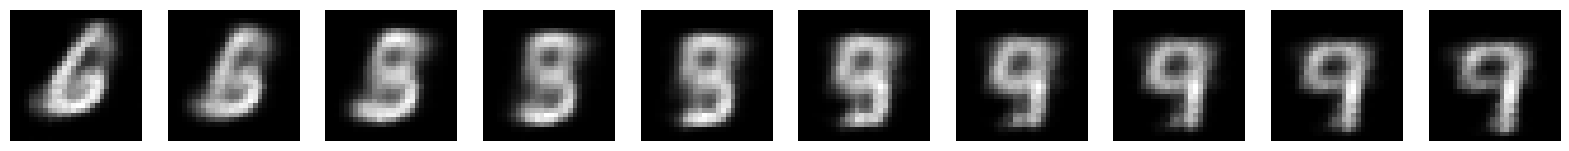
\includegraphics[width=1\linewidth]{report_images/gaussian_vae/interpolation.png}
\caption{\label{fig:inter_guassian}Interpolation: $\mathcal{N}(1,2)$ Prior}
\end{figure}

\noindent
Both the VAEs visually seem to have the same performance producing strong and sharp 0's and 1's and distinguishable 9's while losing its performance for other digits.

%%%%%%%%%%%%%%%%%%%%%%%%%%%%%%%%%%%%%%%%%%%%%%%
\section{Improving Generations}
\subsection{Kaiming Normal Initializaton}
Kaiming Normal initialization optimizes weight initialization for layers with ReLU activations, preventing gradient issues in deep neural networks. Kaiming Normal initialization sets the initial weights $W$ from a normal distribution $W \sim \mathcal{N}(0, \sigma^2)$ where:

\begin{equation}
\sigma = \sqrt{\frac{2}{n_{\text{in}}}}
\end{equation}
where $n_{\text{in}}$ represents the number of input units to a layer.

\begin{figure}[h]
\centering
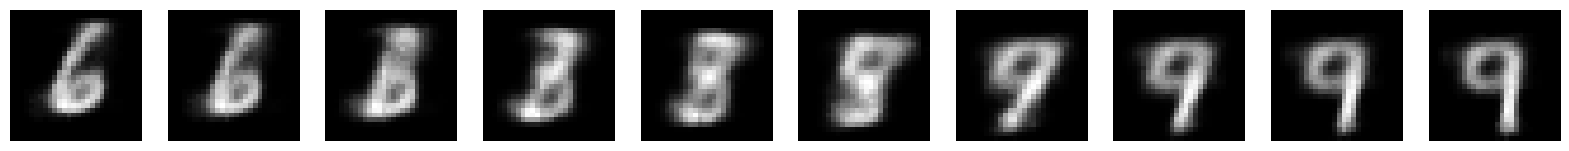
\includegraphics[width=1\linewidth]{report_images/kaiming_init/interpolation.png}
\caption{\label{fig:inter_kaiming}Interpolation: Kaiming Initialization}
\end{figure}

The latent space generations and interpolations seem to be slightly better due to the encoder and decoder both having ReLU activations for its layers. The subsequent models are initialized this way. (Latent space plot: Fig \ref{fig:latent_kaiming}).

\subsection{MSE Loss as Reconstruction Loss}
Mean Squared Error (MSE) loss in Variational Autoencoders (VAEs) quantifies the pixel-wise square of the difference between the original and reconstructed data.

\begin{equation}
\text{MSE} = \|\mathbf{x} - \hat{\mathbf{x}}\|^2_2
\end{equation}
\noindent
where $\mathbf{x}$ is the original data point, and $\hat{\mathbf{x}}$ is the reconstructed data point.

\begin{figure}[h]
\centering
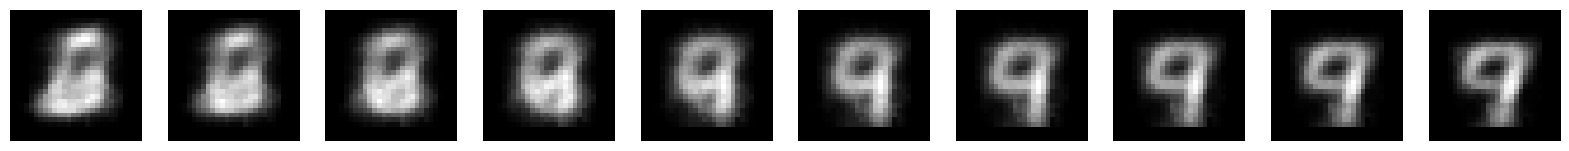
\includegraphics[width=1\linewidth]{report_images/mse/interpolation.png}
\caption{\label{fig:inter_mse}Interpolation: MSE Loss}
\end{figure}
\noindent
The generations (Fig \ref{fig:inter_mse} and Fig \ref{fig:latent_mse}) are blurrier and more faded than the ones of BCE Loss. This can be attributed to the fact that the square of the pixel-wise error can lead to a smoother gradient in the loss landscape, thus minimizing the penalty for small deviations.

\subsection{MAE Loss as Reconstruction Loss}
The Mean Absolute Error (MAE) Loss, also known as L1 loss, is defined to quantify the average magnitude of the absolute differences between original and reconstructed data. It is formulated as:

\begin{equation}
\text{MAE} = \sum_{i=1}^{N} |\mathbf{x}_i - \hat{\mathbf{x}}_i|,
\end{equation}
\noindent
where \(N\) denotes the total number of pixels in an image, $\mathbf{x}$ represents the original image, and $\hat{\mathbf{x}}$ denotes the reconstructed image.

\begin{figure}[h]
\centering
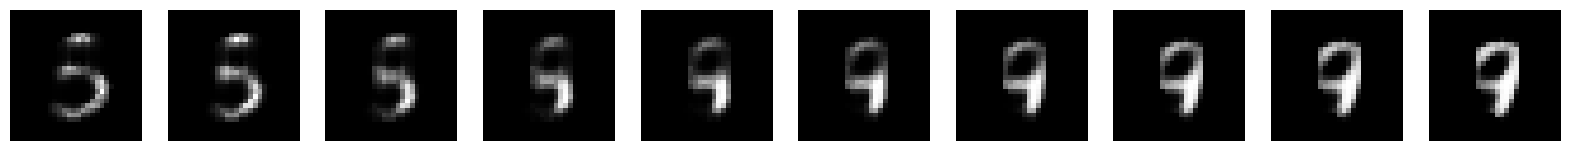
\includegraphics[width=1\linewidth]{report_images/mae/interpolation.png}
\caption{\label{fig:inter_mae}Interpolation: MAE Loss}
\end{figure}
\noindent
Samples (Fig \ref{fig:inter_mae}) using MAE Loss are sharper as MAE directly measures absolute error. Since we are working with values between 0 and 1, it avoids the diminishing effect MSE has due to squaring. 

MAE’s insensitivity to outliers, unlike BCE and MSE, results in less varied, detailed reconstructions, as it tends to gloss over the finer details that contribute significantly to the overall image quality. (Latent space plot: \ref{fig:latent_mae}).

\subsection{Perceptual Loss as Reconstruction Loss}

Perceptual loss (Fig \ref{fig:inter_percep} and Fig \ref{fig:latent_percep}) alone fails to give good samples of our digits since it prioritizes perceptual, higher-level features over pixel-wise reconstruction. Therefore, I paired it with BCE and MSE losses to get better samples.

\begin{figure}[h]
\centering
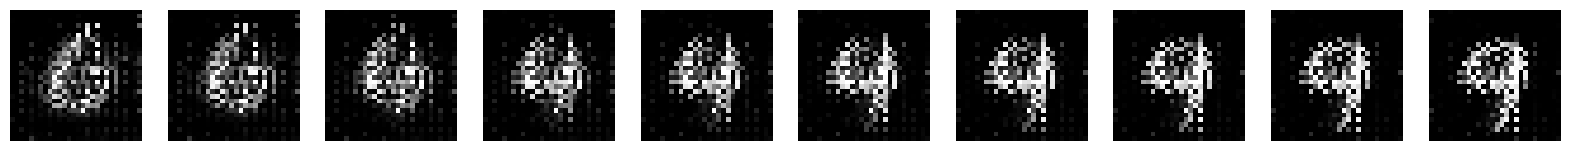
\includegraphics[width=1\linewidth]{report_images/percep/interpolation.png}
\caption{\label{fig:inter_percep}Interpolation: Perceptual Loss}
\end{figure}
\FloatBarrier



\subsection{Weighted Perceptual with BCE Loss as Reconstruction Loss}
Pairing BCE Loss with Perceptual Loss gives us more coherent samples with lesser artefacts (Fig \ref{fig:inter_percep_bce}). It also is able to produce more varied samples unlike BCE Loss - good 7's and even 2's (Fig \ref{fig:latent_percep_bce}) since the perceptual loss component is able to help the model focus on the overall structure of the digits and not only the pixels it consists of.

\begin{figure}[h]
\centering
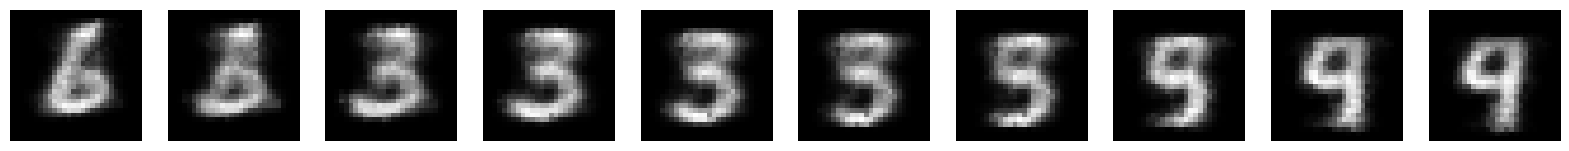
\includegraphics[width=1\linewidth]{report_images/percep_bce/interpolation.png}
\caption{\label{fig:inter_percep_bce}Interpolation: Perceptual Loss with BCE}
\end{figure}

\subsection{Weighted Perceptual Loss with MSE Loss as Reconstruction Loss}
Like perceptual loss paired with BCE, perceptual loss with MSE is able to produce varied results. But its generations are more blurred and less distinct like the generations from the model with just MSE Loss.

\begin{figure}[h]
\centering
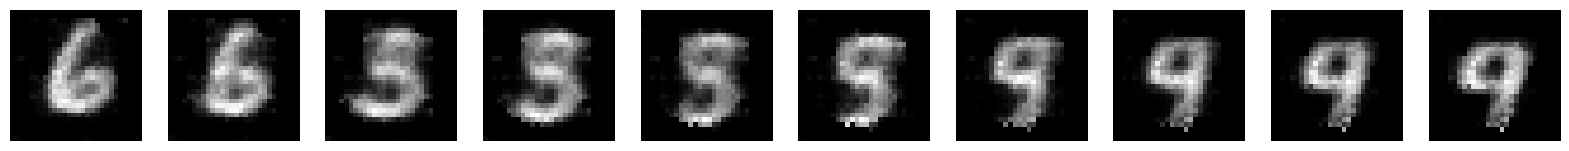
\includegraphics[width=1\linewidth]{report_images/percep_mse/interpolation.png}
\caption{\label{fig:inter_percep_mse}Interpolation: Perceptual Loss with MSE}
\end{figure}

\subsection{BCE Loss for MNIST}
For many image reconstruction tasks, MSE Loss is the go-to choice due to its effectiveness at reducing pixel-level intensity differences. However, for the MNIST dataset, with its images that are essentially binary, BCE Loss is favored. This preference stems from BCE's proficiency in binary classification challenges, making it superior to MSE for distinguishing the stark, black-and-white contrast inherent in MNIST digits.

%%%%%%%%%%%%%%%%%%%%%%%%%%%%%%%%%%%%%%%%%%%%%%%

\section{Reconstructions}
I compare reconstructions of BCE Loss (Fig \ref{fig:recon_bce}) and Perceptual Loss with BCE (Fig \ref{fig:recon_percep_bce}) in this section. Like discussed in the previous section, perceptual loss makes model generation more varied. 

\begin{figure}[h]
\centering
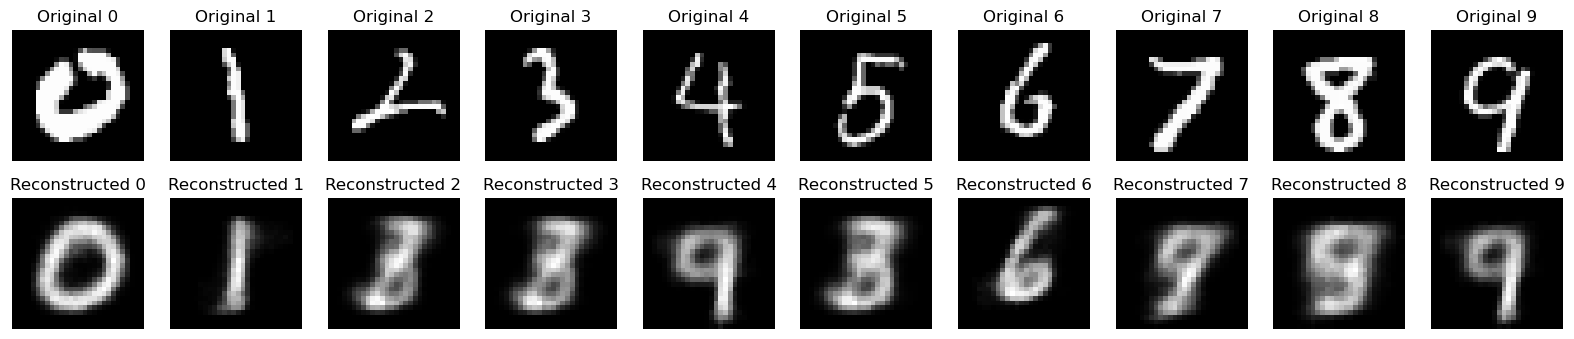
\includegraphics[width=1\linewidth]{report_images/kaiming_init/reconstruction.png}
\caption{\label{fig:recon_bce}Reconstruction: BCE Loss}
\end{figure}

\begin{figure}[h]
\centering
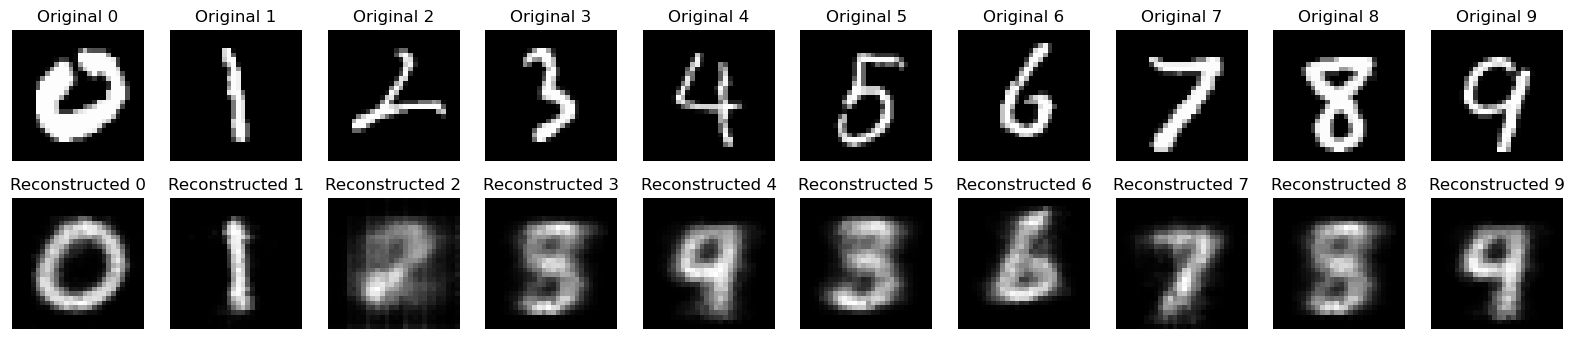
\includegraphics[width=1\linewidth]{report_images/percep_bce/reconstruction.png}
\caption{\label{fig:recon_percep_bce}Reconstruction: Perceptual Loss with BCE}
\end{figure}

%%%%%%%%%%%%%%%%%%%%%%%%%%%%%%%%%%%%%%%%%%%%%%%

\section{Higher Dimensional Latent Spaces}
Two-dimensional latent space offers a very compact representation which may be too limited for capturing the complexity of the dataset. So, I trained a VAE with BCE Loss on a 10 dimensional latent space.. 
\begin{figure}[h]
\centering
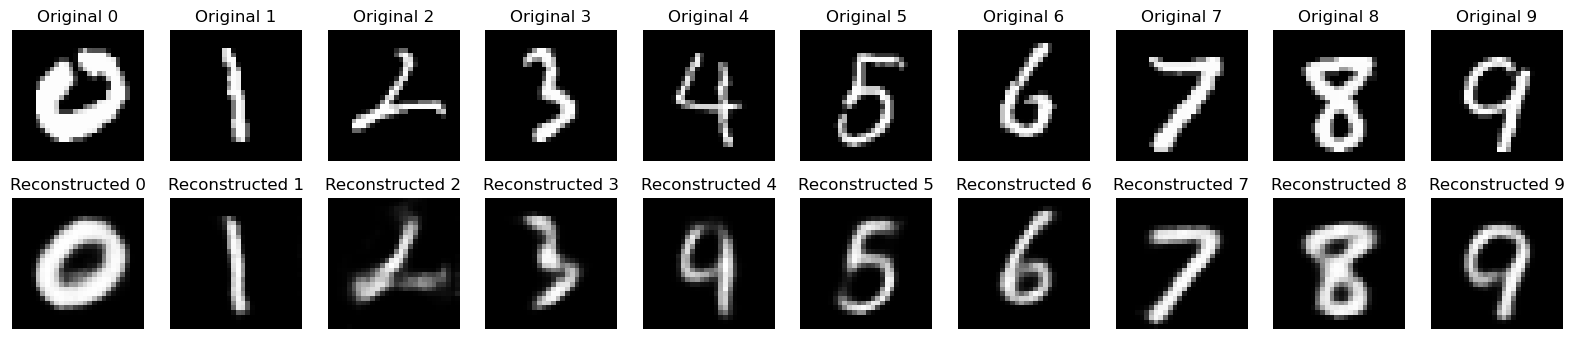
\includegraphics[width=1\linewidth]{report_images/bce_10D/reconstruction.png}
\caption{\label{fig:recon_bce_10D}Reconstruction: BCE Loss - 10D Latent Space}
\end{figure}

\noindent
Reconstructions improves dramatically (Fig \ref{fig:recon_bce_10D} and Fig \ref{fig:inter_bce_10D}) with almost negligible parameters hike - 0.546\%. Original parameter count is 210,821.

\begin{figure}[h]
\centering
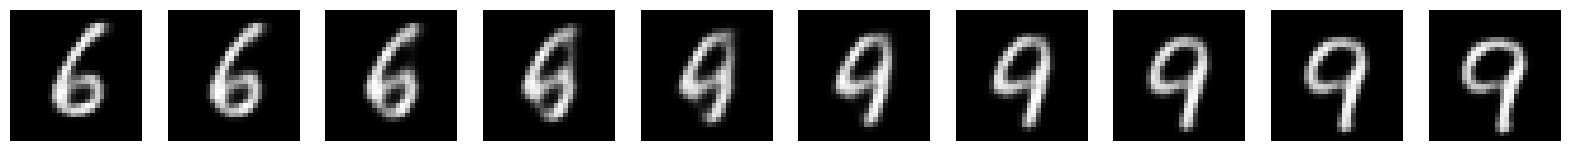
\includegraphics[width=1\linewidth]{report_images/bce_10D/interpolation.png}
\caption{\label{fig:inter_bce_10D}Interpolation: BCE Loss - 10D Latent Space}
\end{figure}
\FloatBarrier




%%%%%%%%%%%%%%%%%%%%%%%%%%%%%%%%%%%%%%%%%%%%%%%
\section{FID Score}
The Fréchet Inception Distance (FID) score quantifies the similarity between generated and real images, utilizing feature vectors extracted from an intermediate layer of the Inception v3 network. A lower FID indicates closer resemblance a more realistic generation. The FID score is calculated as:

\begin{equation}
\text{FID} = \|\boldsymbol{\mu_r} - \boldsymbol{\mu_g}\|^2_2 + \text{Tr}(\boldsymbol{\Sigma_r} + \boldsymbol{\Sigma_g} - 2(\boldsymbol{\Sigma_r\Sigma_g})^{1/2}),
\end{equation}
where $ \boldsymbol{\mu_r}$, $\boldsymbol{\Sigma_r}$ and $\boldsymbol{\mu_g}$, $\boldsymbol{\Sigma_g}$ are the mean vectors and covariance matrices of the real and generated images' feature vectors from the Inception v3 network's intermediate layer, respectively.

\subsection{Implementation}
I used the \textbf{activations} of the \textbf{Mixed-7c layer} of the Inception v3 model to get feature maps of our images.

For each VAE, I \textbf{generated random samples} the size of the MNIST test dataset which is \textbf{10,000 images}, \textbf{resized} them to \textbf{299$\times$299}, \textbf{normalize} the values to be be \textbf{between -1 and 1}, added two extra channels with the same pixels and got our outputs from the model.
\subsection{Results}
\begin{table}[ht]
\centering
\begin{tabular}{@{}lc@{}}
\toprule
VAE Model & FID Score \\ \midrule
\(\mathcal{N}(0,1)\) & 131.7012 \\
\(\mathcal{N}(1,2)\) & 132.0186 \\ 
Kaiming Initialization - BCE Loss & 150.64744\\
MSE Loss & 143.3465 \\ 
MAE Loss & 98.2500 \\
Perceptual Loss & 323.5575\\
Perceptual Loss - BCE Loss & 180.7325 \\
Perceptual Loss - MSE Loss & 176.8897\\ 
10D Latent Space - BCE Loss & 79.7245\\ \bottomrule
\end{tabular}
\caption{\label{tab:FID Baseline}FID Scores of All Models}
\end{table}

\section{Conclusion}
There are a host of other strategies like beta-VAEs, adding noise to the image, using skip connections in forward functions that we can use to get better generations. These were just some popular techniques I used in an attempt to improve samples from \(\mathcal{N}(1,2)\) distribution.

\section{KL Divergence with $\boldsymbol{\mathcal{N}(1,2)}$ Prior}
\label{derivation}
Equation for multivariate gaussian:
\begin{equation}
\mathcal{N}(\mathbf{x};\boldsymbol{\mu},\boldsymbol{\Sigma})=
\frac{1}{2^{n/2} |\boldsymbol{\Sigma}|}\exp \left(
-\frac{1}{2} (\mathbf{x}-\boldsymbol{\mu})^{\intercal}  \boldsymbol{\Sigma}^{-1}(\mathbf{x}-\boldsymbol{\mu})
\right)
\end{equation}
where $\mathbf{x},\boldsymbol{\mu}\in\mathbb{R}^n$ and $\boldsymbol{\Sigma}\in\mathbb{R}^{n\times n}$. 

We assume that the mean is vector of 1's and the covariance is a diagonal matrix of 4's. (I am taking second parameter of $\mathcal{N}$ to be variance in this derivation, as opposed to the standard practice in this report). Therefore:
$$
p_1 = q_\phi(\mathbf{z}|\mathbf{x}) = \mathcal{N}(\boldsymbol{\mu}_1,\boldsymbol{\Sigma}_1) = \mathcal{N}(\boldsymbol{\mu},\boldsymbol{\sigma}^2)
$$
where $\boldsymbol{\mu}$ and $\boldsymbol{\sigma}$ are the mean and standard deviation vectors of the surrogate posterior, and
$$p_2 = p_\theta(\mathbf{z}) =\mathcal{N}(\boldsymbol{\mu}_2,\boldsymbol{\Sigma}_2) =\mathcal{N}(\mathbf{1},\mathbf{4})$$ 
Therefore, $D_{KL}\left(q_\phi(\mathbf{z}|\mathbf{x}) || p_\theta(\mathbf{z})\right) $ can be written as
\[
\begin{split}
& \frac{1}{2} \left[ \log\frac{|\boldsymbol{\Sigma}_2|}{|\boldsymbol{\Sigma}_1|} - n + \text{tr}(\boldsymbol{\Sigma}_2^{-1}\boldsymbol{\Sigma}_1) + (\boldsymbol{\mu}_2 - \boldsymbol{\mu}_1)^\intercal \boldsymbol{\Sigma}_2^{-1}(\boldsymbol{\mu}_2 - \boldsymbol{\mu}_1) \right] \\
& = \frac{1}{2}\left[ \log\frac{2^{2n}}{|\boldsymbol{\Sigma}_1|} - n + \frac{1}{4} \text{tr}(\boldsymbol{\Sigma}_1) + \frac{1}{4}(\mathbf{1} - \boldsymbol{\mu})^\intercal(\mathbf{1} - \boldsymbol{\mu}) \right] \\
& = \frac{1}{2}\left[ 2n\log2 - \sum_{j=1}^n \log\sigma_j^2 - n + \frac{1}{4}\sum_{j=1}^n \sigma_j^2 + \frac{1}{4}\sum_{j=1}^n (1 - \mu_j)^2 \right] \\
& = -\frac{1}{2}\sum_{j=1}^n \left[ 1 - 2\log2 + \log\sigma_j^2  - \frac{1}{4}\sigma_j^2 - \frac{1}{4}(1 - \mu_j)^2 \right]
\end{split}
\]
Hence, proved.

\pagebreak


%%%%%%%%%%%%%%%%%%%%%%%%%%%%%%%%%%%%%%%%%%%%%%%

\section{Latent Space Plots}
\label{latent_spaces}
\begin{figure}[h]
\centering
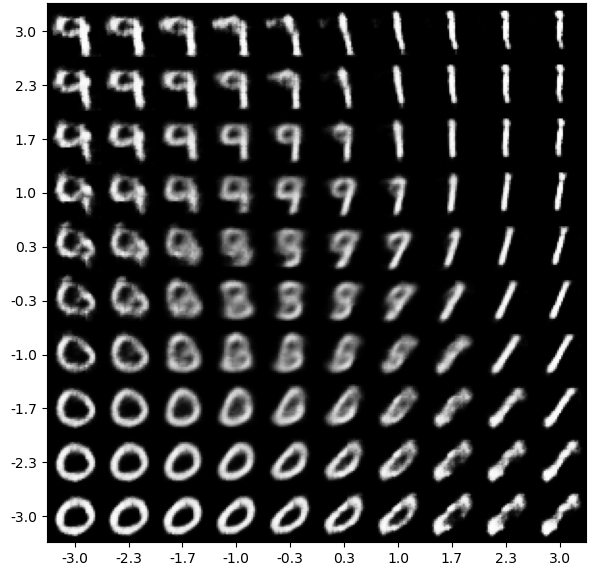
\includegraphics[width=1\linewidth]{report_images/normal_vae/latent_space.png}
\caption{\label{fig:latent_normal}Latent Space: $\mathcal{N}(0,1)$ Prior}
\end{figure}

\begin{figure}[h]
\centering
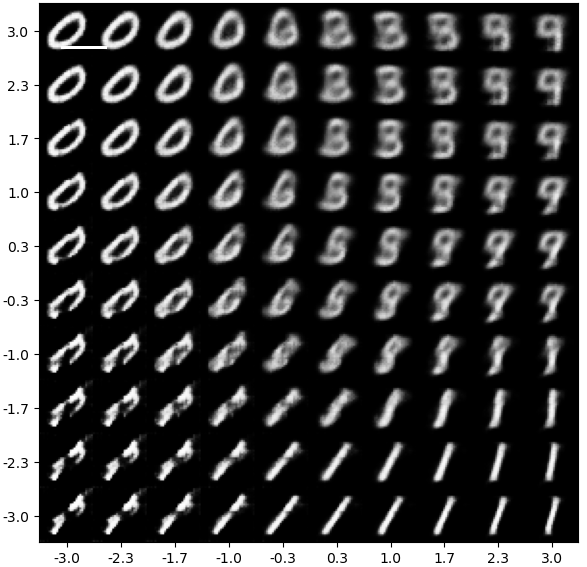
\includegraphics[width=1\linewidth]{report_images/gaussian_vae/latent_space.png}
\caption{\label{fig:latent_guassian}Latent Space: $\mathcal{N}(1,2)$ Prior}
\end{figure}

\begin{figure}[h]
\centering
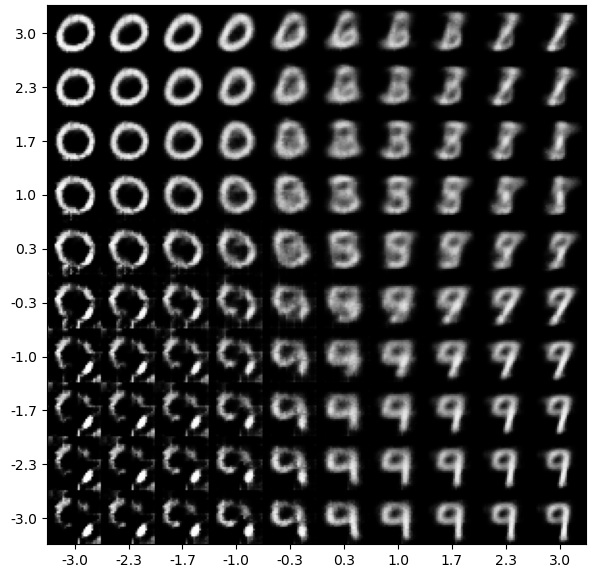
\includegraphics[width=1\linewidth]{report_images/kaiming_init/latent_space.png}
\caption{\label{fig:latent_kaiming}Latent Space: Kaiming Initialization with BCE Loss}
\end{figure}

\begin{figure}[h]
\centering
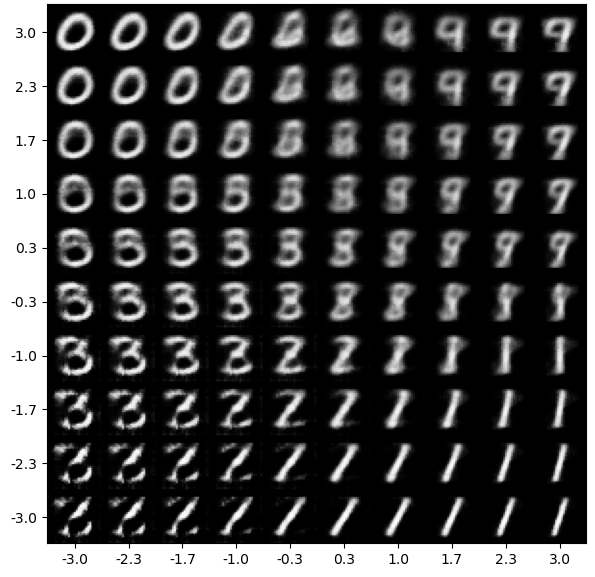
\includegraphics[width=1\linewidth]{report_images/mse/latent_space.png}
\caption{\label{fig:latent_mse}Latent Space: MSE Loss}
\end{figure}

\begin{figure}[h]
\centering
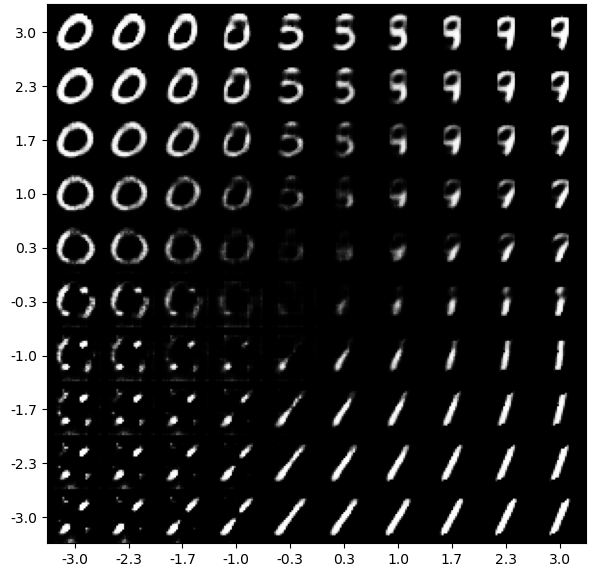
\includegraphics[width=1\linewidth]{report_images/mae/latent_space.png}
\caption{\label{fig:latent_mae}Latent Space: MAE Loss}
\end{figure}

\begin{figure}[h]
\centering
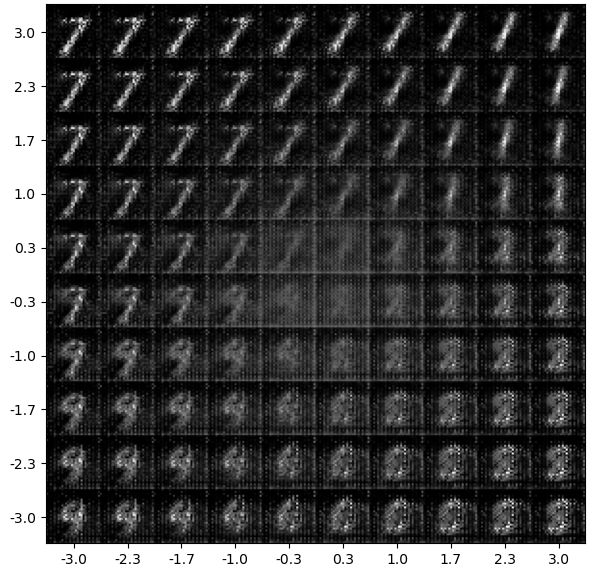
\includegraphics[width=1\linewidth]{report_images/percep/latent_space.png}
\caption{\label{fig:latent_percep}Latent Space: Perceptual Loss}
\end{figure}

\begin{figure}[h]
\centering
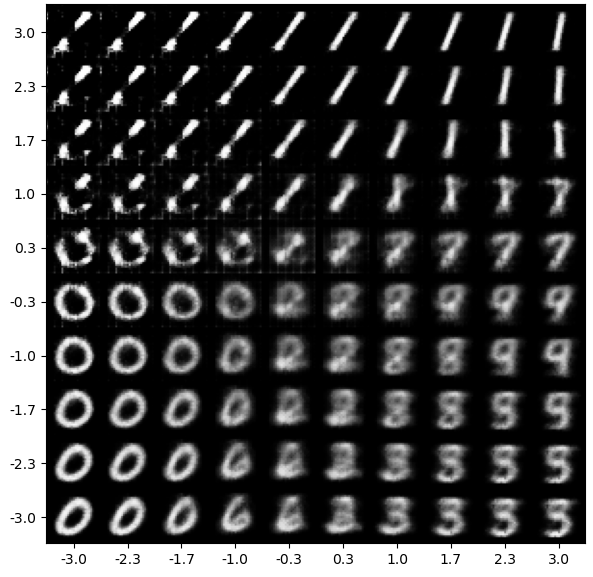
\includegraphics[width=1\linewidth]{report_images/percep_bce/latent_space.png}
\caption{\label{fig:latent_percep_bce}Latent Space: Perceptual Loss with BCE}
\end{figure}

\begin{figure}[h]
\centering
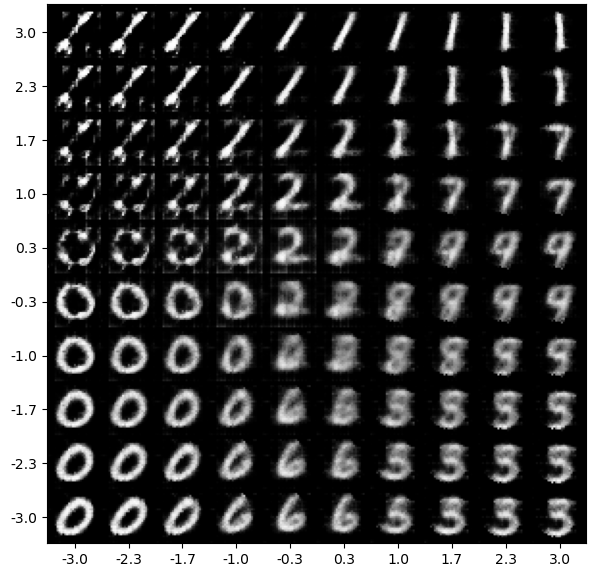
\includegraphics[width=1\linewidth]{report_images/percep_mse/latent_space.png}
\caption{\label{fig:latent_percep_mse}Latent Space: Perceptual Loss with MSE}
\end{figure}

\end{document}